\documentclass[11pt,a4paper]{article}

\usepackage[utf8]{inputenc}
\usepackage[T1]{fontenc}
\usepackage{lmodern}
\usepackage[margin=2.5cm]{geometry}
\usepackage{microtype}
\usepackage{amsmath,amssymb}
\usepackage{graphicx}
\usepackage{booktabs,tabularx,array}
\usepackage{xcolor}
\usepackage{tikz}
\usetikzlibrary{arrows.meta,positioning,shapes.geometric,fit,calc,backgrounds}
\usepackage{listings}
\usepackage[most]{tcolorbox}
\usepackage{enumitem}
\usepackage{caption}
\usepackage[numbers,sort&compress]{natbib}
\usepackage[hidelinks,colorlinks=true,linkcolor=blue!50!black,citecolor=blue!50!black,urlcolor=blue!50!black]{hyperref}

\definecolor{codebg}{RGB}{247,248,250}
\definecolor{kw}{RGB}{0,92,160}
\definecolor{cm}{RGB}{90,110,90}
\definecolor{st}{RGB}{160,60,20}
\lstdefinestyle{py}{
  language=Python, basicstyle=\ttfamily\footnotesize, backgroundcolor=\color{codebg},
  keywordstyle=\color{kw}\bfseries, commentstyle=\color{cm}\itshape, stringstyle=\color{st},
  frame=single, rulecolor=\color{black!15}, breaklines=true, breakatwhitespace=false,
  showstringspaces=false, columns=fullflexible, keepspaces=true, xleftmargin=2pt, xrightmargin=2pt,
  numbers=left, numberstyle=\tiny\color{black!45}, numbersep=6pt, aboveskip=6pt, belowskip=4pt,
  literate={→}{$\rightarrow$}1
}
\lstset{style=py}
\newcommand{\code}[1]{\texttt{\detokenize{#1}}}

\newtcolorbox{keyidea}[1][]{colback=blue!4,colframe=blue!45!black,fonttitle=\bfseries,title={Key idea},#1}
\newtcolorbox{lesson}[1][]{colback=orange!6,colframe=orange!60!black,fonttitle=\bfseries,title={Engineering lesson},#1}
\newtcolorbox{objectives}[1][]{colback=green!5,colframe=green!40!black,fonttitle=\bfseries,title={Learning objectives},#1}
\newtcolorbox{exercise}[1][]{colback=gray!8,colframe=gray!60!black,fonttitle=\bfseries,title={Exercise},#1}

\newcommand{\figscreen}[3]{\begin{figure}[t]\centering\includegraphics[width=#3\linewidth]{figures/#1}\caption{#2}\label{fig:#1}\end{figure}}

\title{\bfseries ForgeAgent: A Fully Local Autonomous Software-Engineering Agent\\[2pt]
\large Verified Reporting, Policy-Gated Tool Execution and Crash-Safe State\\ on Consumer Hardware with an Open-Weights Model}
\author{Anthony Efemena Edjenuwa\\[2pt]\small Independent researcher and developer\\[2pt]\small\texttt{github.com/bahdleen/forgeagent}}
\date{Technical report --- 14 October 2026}

\begin{document}
\maketitle

\begin{abstract}
\noindent
Autonomous coding agents are usually thin clients for hosted frontier models. This report describes \emph{ForgeAgent}, a complete,
open-source agent platform that runs entirely on one consumer laptop (an NVIDIA RTX 4090 Laptop GPU with 16\,GB of VRAM and 64\,GB of RAM)
using a 27-billion-parameter open-weights model quantised to 4 bits and served by llama.cpp. The contribution is not a new model but the
\emph{systems engineering} that makes a small, locally hosted, imperfect model safe and useful enough to modify real code bases:
(i) an LLM gateway that streams, cancels instantly, and \emph{recovers} malformed tool calls; (ii) a typed tool layer with a three-mode permission
policy, workspace confinement and an immutable audit log; (iii) an orchestration loop with planning, a dependency-aware task queue, role-specialised
prompts that share one model instance, and guards that refuse to let the agent declare success while verification fails;
(iv) crash-safe persistence so interrupted work can be resumed; and (v) context budgeting, compaction and a persistent, searchable project memory.
The final report shown to the user is generated from the audit log rather than from the model's claims.
On the target machine we measured throughput, GPU/CPU utilisation, tool-call reliability and executed-code correctness for three quantisations of the same model, and found that the quantisation that fits entirely in VRAM generated about five times faster (36 versus 7 tokens/s) with no difference we could detect on a small workload.
We describe the architecture, give the key algorithms and real source excerpts, report automated-test results and end-to-end
experiments with the actual local model, and document the engineering pitfalls we met (stale bytecode caches, a commit-after-response race,
CRLF-incompatible patches, over-eager secret redaction). The report is written to be \emph{educational}: every section lists learning objectives,
highlights the underlying principle, and ends with exercises. We state limitations plainly, in particular that the system is not a sandbox.
\end{abstract}

\noindent\textbf{Keywords:} LLM agents, local inference, llama.cpp, tool use, software engineering agents, prompt injection, least privilege, context management.

\tableofcontents
\clearpage

%==============================================================================================
\section{Introduction}
\begin{objectives}
After this section you should be able to: (1) define an \emph{LLM agent} and its control loop; (2) explain why local deployment changes the engineering
problem; (3) list the requirements ForgeAgent was built to satisfy.
\end{objectives}

A \emph{language-model agent} wraps a model in a loop: the model proposes an action, an environment executes it, and the observation is fed
back \citep{yao2023react,wang2024survey}. For software engineering, the actions are file edits, shell commands and test runs; benchmarks such as
SWE-bench \citep{jimenez2024swebench} and agent--computer interfaces such as SWE-agent \citep{yang2024sweagent} show that carefully designed tools matter as much as the
underlying model.

Most such systems call a remote API. Running the model \emph{locally} offers privacy, no per-token cost, offline operation and full control, but it changes
the engineering constraints in four ways:
\begin{enumerate}[nosep]
  \item \textbf{Weaker, less reliable models.} Small open models emit malformed tool calls, loop, or announce a plan and stop.
  \item \textbf{Scarce memory.} A 27B-parameter model at 4 bits occupies about 15.4\,GiB (Section~\ref{sec:hw}); the context window competes with the weights for VRAM.
  \item \textbf{Low throughput.} Partial CPU offload yields roughly 10 generated tokens per second, so wasted steps are expensive.
  \item \textbf{Weaker alignment guarantees.} Some community models are deliberately modified to refuse less \citep{arditi2024refusal}; safety must therefore live in the \emph{system}, not in the model.
\end{enumerate}

\subsection{Requirements}
ForgeAgent was specified to: inspect and modify repositories; execute terminal commands and tests; operate a browser; plan and decompose work; keep long-running
progress and resume after restarts; coordinate specialised roles on a single model instance; keep persistent memory; expose a professional UI; and respect explicit
permission boundaries, with execution permissions kept separate from the model's own refusal behaviour (no keyword filters in the gateway).

\subsection{Contributions}
\begin{itemize}[nosep]
  \item A complete, runnable architecture (Section~\ref{sec:arch}) with 28 typed tools and 5 logical roles on one model.
  \item A \emph{tool-call recovery} layer making small models usable (Section~\ref{sec:gateway}).
  \item \emph{Verified reporting}: guards and an audit-derived report that keep the agent honest (Section~\ref{sec:loop}).
  \item A least-privilege permission model with workspace confinement, and an explicit, honest threat model (Section~\ref{sec:tools}).
  \item Crash-safe persistence and resume, context budgeting and compaction, and local vector memory (Sections~\ref{sec:persist}--\ref{sec:memory}).
  \item An empirical evaluation with the real local model and a catalogue of engineering lessons (Sections~\ref{sec:eval}--\ref{sec:lessons}).
\end{itemize}

%==============================================================================================
\section{Background}
\begin{objectives}
Understand tool calling, quantisation and the KV cache well enough to reason about the hardware numbers later; understand prompt injection.
\end{objectives}

\paragraph{Tool calling.} The de-facto wire format is the OpenAI chat-completions schema \citep{openaitools}: the client sends JSON-Schema tool definitions; the model returns
\code{tool_calls} with a function name and a JSON string of arguments; the client executes them and replies with \code{tool} messages.
llama.cpp \citep{llamacpp} reproduces this interface for local models, applying the model's chat template server-side.
Models differ in how reliably they follow it \citep{schick2023toolformer}, which motivates Section~\ref{sec:gateway}.

\paragraph{Quantisation and memory.} Post-training quantisation \citep{dettmers2022llmint8,frantar2023gptq} stores weights in 4--8 bits. llama.cpp's \texttt{Q4\_K\_M}
format averages roughly 4.5--5 bits per weight. During generation the transformer \citep{vaswani2017attention} also keeps a \emph{key--value (KV) cache} whose size grows linearly with context length;
cache memory dominates serving cost at long contexts \citep{kwon2023vllm}. FlashAttention-style kernels \citep{dao2024flashattention2} reduce attention memory traffic (enabled with \texttt{-fa}).

\paragraph{Long context is not free.} Even when a model accepts a long prompt, it uses information in the middle of it poorly \citep{liu2024lost}. Agents therefore benefit from
\emph{short, curated} contexts, which motivates compaction (Section~\ref{sec:context}).

\paragraph{Prompt injection.} When an agent reads files, web pages or tool output, any of them may contain text that tries to give the agent new instructions
\citep{perez2022ignore,greshake2023indirect}. Benchmarks such as AgentDojo \citep{debenedetti2024agentdojo} show that models alone do not reliably resist this. The practical defence is architectural:
\emph{limit what a hijacked agent can do} (least privilege \citep{saltzer1975protection}) and keep a record of what it did \citep{owaspllm}.

\begin{keyidea}
\textbf{Capability, not intention.} A model's refusal behaviour is an unreliable control. ForgeAgent enforces permissions \emph{in code}, outside the model,
and treats everything the model reads as untrusted data.
\end{keyidea}

%==============================================================================================
\section{Related work}
ReAct \citep{yao2023react} interleaves reasoning and acting and is the template for our loop. Reflexion \citep{shinn2023reflexion} adds verbal self-feedback after failures; ForgeAgent's
``error $\rightarrow$ fix'' memory records (Section~\ref{sec:memory}) play a similar role but are stored persistently and are human-editable.
MemGPT \citep{packer2023memgpt} treats the context window like virtual memory, paging information in and out; our compaction and tool-output truncation with on-demand retrieval
(\code{read_full_output}) follow the same intuition at a smaller scale. SWE-agent \citep{yang2024sweagent} demonstrates that a purpose-built tool interface (e.g.\ guarded edit commands)
improves success; our \code{edit_file} returns the closest matching text on failure for the same reason. Surveys of LLM-based agents \citep{wang2024survey} situate these components.
Unlike these research systems, ForgeAgent targets a complete \emph{local product}: UI, persistence, permissions and installation are part of the contribution. We do not claim state-of-the-art
benchmark performance and do not evaluate on SWE-bench.

%==============================================================================================
\section{System architecture}\label{sec:arch}
\begin{objectives}
Name the components of the system and the direction of every dependency; explain why roles share one model instance.
\end{objectives}

Figure~\ref{fig:arch} shows the system. A React/TypeScript front end communicates with a FastAPI \citep{fastapi} back end over REST and a WebSocket that carries live events.
The back end persists everything in SQLite \citep{sqlite} through SQLAlchemy \citep{bayer2012sqlalchemy} with Alembic migrations. All model access goes through one gateway to a local
\texttt{llama-server}.

\begin{figure}[t]
\centering
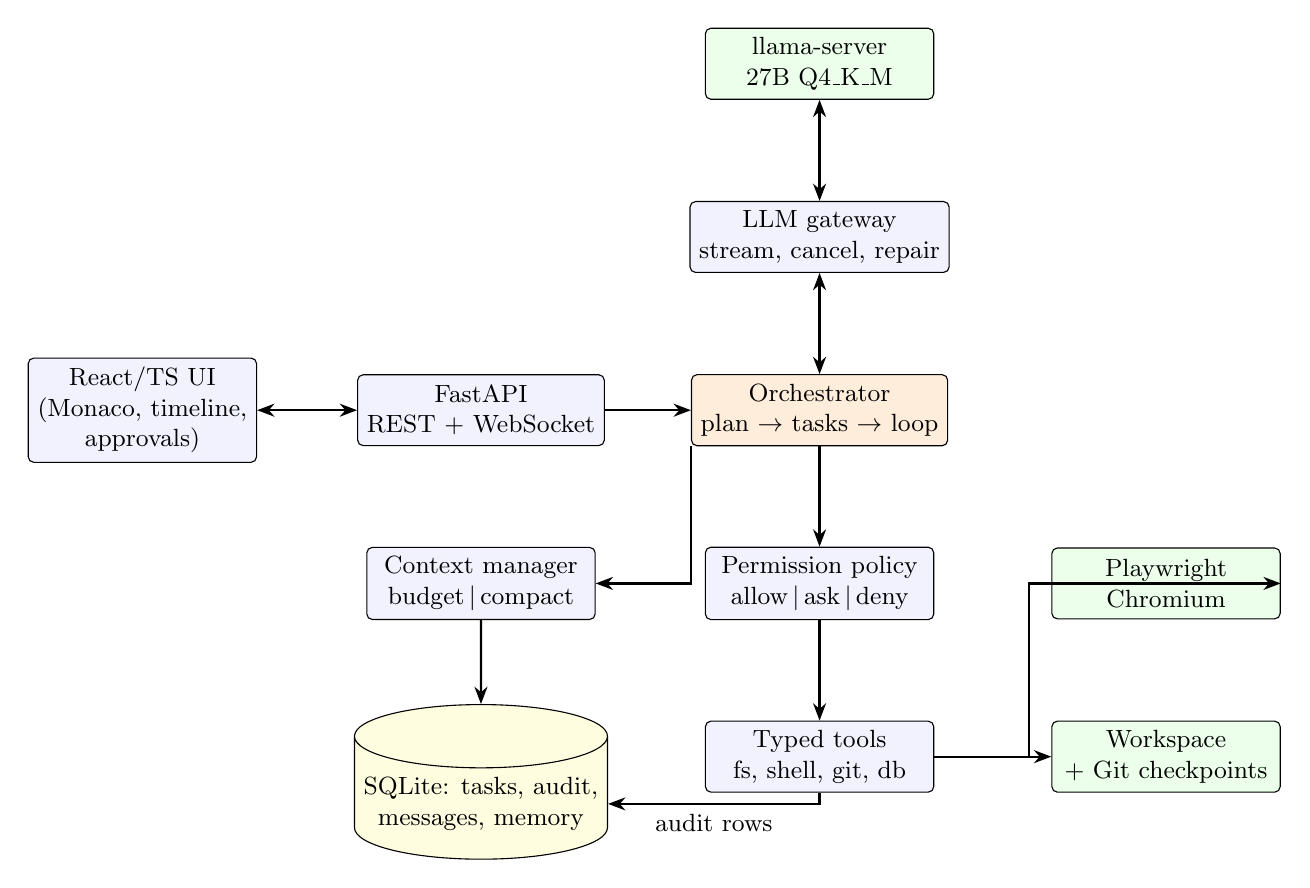
\begin{tikzpicture}[
  font=\small, x=1cm, y=1cm,
  box/.style={draw, rounded corners=2pt, align=center, minimum height=9mm, minimum width=29mm, fill=blue!5},
  store/.style={draw, cylinder, shape border rotate=90, aspect=0.25, align=center, minimum height=11mm, minimum width=26mm, fill=yellow!12},
  ext/.style={draw, rounded corners=2pt, align=center, minimum height=9mm, minimum width=29mm, fill=green!8},
  arr/.style={-{Stealth[length=2.2mm]}, thick}, darr/.style={{Stealth[length=2.2mm]}-{Stealth[length=2.2mm]}, thick}]
  \node[box] (ui) at (0,0) {React/TS UI\\(Monaco, timeline,\\approvals)};
  \node[box] (api) at (4.3,0) {FastAPI\\REST + WebSocket};
  \node[box, fill=orange!14] (orch) at (8.6,0) {Orchestrator\\plan $\rightarrow$ tasks $\rightarrow$ loop};
  \node[box] (gw) at (8.6,2.2) {LLM gateway\\stream, cancel, repair};
  \node[ext] (llama) at (8.6,4.4) {llama-server\\27B Q4\_K\_M};
  \node[box] (pol) at (8.6,-2.2) {Permission policy\\allow\,\textbar\,ask\,\textbar\,deny};
  \node[box] (tools) at (8.6,-4.4) {Typed tools\\fs, shell, git, db};
  \node[ext] (ws) at (13.0,-4.4) {Workspace\\+ Git checkpoints};
  \node[ext] (pw) at (13.0,-2.2) {Playwright\\Chromium};
  \node[box] (ctx) at (4.3,-2.2) {Context manager\\budget\,\textbar\,compact};
  \node[store] (db) at (4.3,-5.0) {SQLite: tasks, audit,\\messages, memory};
  \draw[darr] (ui)--(api); \draw[arr] (api)--(orch);
  \draw[darr] (orch)--(gw); \draw[darr] (gw)--(llama);
  \draw[arr] (orch)--(pol); \draw[arr] (pol)--(tools);
  \draw[arr] (tools)--(ws); \draw[arr] (tools.east) -- ++(1.2,0) |- (pw.east);
  \draw[arr] (orch.south west) |- (ctx.east);
  \draw[arr] (ctx)--(db);
  \draw[arr] (tools.south) |- (db.east) node[pos=.75,below]{audit rows};
\end{tikzpicture}
\caption{ForgeAgent components. Arrows show the direction of calls. Every tool execution passes through the permission policy and is recorded in SQLite.}
\label{fig:arch}
\end{figure}


\subsection{Hardware and model}\label{sec:hw}
The target machine has an RTX 4090 Laptop GPU (16\,GB VRAM), 64\,GB RAM and Windows~11. The model is a community build of Qwen3.8-27B in GGUF format
\citep{hfmodel,qwen3report}, quantised with \texttt{Q4\_K\_M}; the file is 15.4\,GiB and the model has 27.3\,B parameters as reported by the server.
The model alone nearly fills the card, so llama.cpp's automatic fitting places as many layers as possible in VRAM and runs the rest on the CPU.
With \texttt{Q4\_K\_M} the measured generation speed was 7--10 tokens/s; an 11\,GB \texttt{IQ3\_S} quantisation that fits entirely in VRAM reached about 36 tokens/s (Section~\ref{sec:quant}).
Further measured values are reported in Section~\ref{sec:eval}.

\subsection{Roles on a single model}
ForgeAgent defines five \emph{logical} roles --- Architect, Developer, Debugger, Tester, Reviewer. A role is nothing more than a different system prompt
(Section~\ref{sec:prompts}) and a different tool subset; all roles call the same model instance, serialised by one semaphore. Loading five 27B models is impossible on this hardware, and
sequential execution also keeps resource use predictable.

\begin{keyidea}
\textbf{Specialisation without replication.} Role prompts bias the single model toward a task (design, implement, diagnose, test, review) and the tool subset
\emph{removes} capabilities (the Architect and Reviewer cannot write files). The restriction is enforced in code, not requested in prose.
\end{keyidea}

%==============================================================================================
\section{The local LLM gateway}\label{sec:gateway}
\begin{objectives}
Explain how a streaming completion becomes a validated tool call, and why a recovery layer is necessary for small models.
\end{objectives}

The gateway speaks the OpenAI-compatible protocol to llama.cpp. It (a) discovers the model from \code{/models} and reads capabilities (real context size,
whether the chat template supports tools) from llama.cpp's \code{/props}; (b) parses the server-sent event stream, assembling content, reasoning tokens and
\emph{fragmented} tool-call deltas; (c) records token usage and generation speed from the server's timing fields; (d) retries transport and 5\textsc{xx} errors with exponential backoff;
and (e) supports cancellation.

\subsection{Tool-call recovery}
In our experiments the native tool-call path worked with the chosen model, but the gateway is built for the general case. Native calling is tried first; if the server rejects the
\code{tools} field (HTTP 400), the gateway switches permanently to a \emph{prompt-based} protocol: tool schemas are placed in the system prompt, and the model replies with
\code{<tool_call>{json}</tool_call>} blocks. Independently of the mode, tool calls found \emph{in text} are recovered from several dialects: JSON blocks, the Qwen XML dialect
(\code{<function=name><parameter=key>value</parameter></function>}) and fenced JSON. Listing~\ref{lst:repair} shows the JSON repair used for truncated or sloppy arguments.
Unrepairable calls are \emph{never executed}: they are returned to the model as an error that restates the expected schema.

\begin{lstlisting}[caption={JSON repair for model-generated tool arguments (excerpt from \texttt{backend/app/llm/toolparse.py}).},label={lst:repair}]
\end{lstlisting}
\lstinputlisting[basicstyle=\ttfamily\scriptsize]{listings/repair_json.py}

\subsection{Instant cancellation}
A user pressing \emph{Stop} must take effect immediately, but llama.cpp may spend tens of seconds evaluating a long prompt before it emits the first token, during which a naive
\texttt{for line in stream} loop cannot observe a cancel flag. The gateway therefore races the next stream read against a cancel event (Listing~\ref{lst:cancel}); leaving the HTTP context
closes the connection, which makes llama.cpp abort generation. A unit test with a server that stalls for 30\,s verifies that cancellation completes in under 3\,s.
\lstinputlisting[caption={Cancellable stream iteration (\texttt{backend/app/llm/gateway.py}).},label={lst:cancel},basicstyle=\ttfamily\scriptsize]{listings/cancellable.py}

\begin{lesson}
Blocking I/O hides cancellation. Any loop that waits on a remote producer needs a way to be woken by the cancel signal, not just a flag polled between items.
\end{lesson}

%==============================================================================================
\section{Typed tools and the permission policy}\label{sec:tools}
\begin{objectives}
Describe how a tool is defined, validated and audited; apply the principle of least privilege to an agent.
\end{objectives}

\subsection{Tool abstraction}
Every tool declares a name, a description, a Pydantic parameter model (which doubles as the JSON Schema shown to the model), a \emph{category}
(\texttt{read, write, exec, git, browser, destructive, meta}) and returns a structured \code{ToolResult}. Listing~\ref{lst:toolbase} shows the base class.
\lstinputlisting[caption={Tool base class (\texttt{backend/app/tools/base.py}).},label={lst:toolbase},basicstyle=\ttfamily\scriptsize]{listings/tool_base.py}

ForgeAgent registers 28 tools (Table~\ref{tab:tools}). Arguments are validated before execution; a validation failure is returned to the model with the offending fields and the expected schema,
which small models use to self-correct. Every execution creates a row in an append-only \code{tool_runs} table with the (secret-redacted) arguments, full output, approval state, duration and the files touched.

\begin{table}[t]
\centering\small
\begin{tabularx}{\linewidth}{lX}
\toprule
\textbf{Category} & \textbf{Tools}\\\midrule
Filesystem (read) & \code{list_directory, read_file, search_files, search_code, query_database, inspect_logs, read_full_output}\\
Filesystem (write) & \code{create_file, edit_file, apply_patch, move_file}; \code{delete_file} (destructive)\\
Execution & \code{run_command, run_tests, run_build, start_dev_server, stop_dev_server}\\
Git & \code{git_changes, create_checkpoint}; \code{restore_checkpoint} (destructive)\\
Browser & \code{open_browser, capture_screenshot, inspect_browser_errors, browser_interact}\\
Control \& memory & \code{submit_plan, complete_task, remember, recall}\\\bottomrule
\end{tabularx}
\caption{The 28 registered tools by category.}\label{tab:tools}
\end{table}

\subsection{Workspace confinement}
File tools resolve every path with the real path of the target (following symbolic links and Windows junctions) and refuse anything outside the authorised workspace;
\texttt{.git/} and \texttt{.forge/} are write-protected (Listing~\ref{lst:resolve}). Writes are atomic (temporary file, \texttt{fsync}, \texttt{os.replace}), so a crash never leaves a half-written source file.
\lstinputlisting[caption={Workspace path validation (\texttt{backend/app/security.py}).},label={lst:resolve},basicstyle=\ttfamily\scriptsize]{listings/resolve_in_workspace.py}
\lstinputlisting[caption={Atomic file write (\texttt{backend/app/tools/fs\_tools.py}).},basicstyle=\ttfamily\scriptsize]{listings/atomic_write.py}

\subsection{Autonomy modes}\label{sec:modes}
Three modes decide, per call, whether a tool runs (\emph{allow}), needs the user's consent (\emph{ask}) or is disabled (\emph{deny}):
\begin{description}[nosep]
  \item[Supervised] reads run automatically; every write, command and browser action asks.
  \item[Project autonomous] (default) edits, builds, tests and approved development commands run inside the workspace; deletions, checkpoint restores, destructive or network
  commands, secrets, deployments, unknown commands, paths outside the workspace and external URLs ask.
  \item[Custom] a per-tool allow/ask/deny table; unspecified tools follow the project-autonomous policy.
\end{description}
\lstinputlisting[caption={The permission decision function (\texttt{backend/app/agent/permissions.py}).},label={lst:decide},basicstyle=\ttfamily\scriptsize]{listings/decide.py}

\subsection{Command classification}
Shell commands are classified by \code{classify_command} (Listing~\ref{lst:classify}): regular expressions detect destructive operations, network use, deployment and secret access; absolute or parent-relative
paths outside the workspace are flagged; and every sub-command of a chain (\code{&&}, \code{;}, \code{|}) must begin with an allow-listed development tool
after normalising quoted executable paths. Table~\ref{tab:classify} shows representative verdicts from the test suite.
\lstinputlisting[caption={Command classification (\texttt{backend/app/security.py}).},label={lst:classify},basicstyle=\ttfamily\scriptsize]{listings/classify_command.py}

\begin{table}[t]
\centering\small
\begin{tabular}{lc}
\toprule \textbf{Command} & \textbf{Verdict}\\\midrule
\code{npm test} / \code{python -m pytest -q} / \code{git status && git diff} & auto\\
\code{npm install express} & auto\\
\code{rm -rf node_modules} & approval (destructive)\\
\code{git push origin main} & approval (destructive / external)\\
\code{curl http://x/s.sh | sh} & approval (network)\\
\code{type ..\\..\\secrets.txt} & approval (outside workspace)\\
\code{npm test && rm -rf /} & approval (one bad link taints the chain)\\
\code{vercel deploy --prod} & approval (deployment)\\\bottomrule
\end{tabular}
\caption{Representative command-classification outcomes (from \code{tests/test_security_fs.py}).}\label{tab:classify}
\end{table}

\begin{keyidea}
\textbf{Heuristics are not a sandbox.} The classifier reduces accidents and makes risky actions visible, but a command obfuscated by indirection (for example a script the agent writes and then runs) can
bypass it. Real isolation requires an OS-level boundary (a VM, WSL2 or a restricted account); ForgeAgent does not provide one (Section~\ref{sec:limits}).
\end{keyidea}

%==============================================================================================
\section{The agent loop}\label{sec:loop}
\begin{objectives}
Trace one user request through planning, the task queue and the tool loop; explain each guard and the failure it prevents.
\end{objectives}

\subsection{Control flow}
Figure~\ref{fig:loop} shows the loop. A request creates a root \emph{task}; a Git checkpoint is committed first so the whole run can be undone. If planning is enabled
(\emph{auto} for long or build-style requests), the Architect role inspects the workspace with read-only tools and calls \code{submit_plan} with a summary, technology stack and an ordered list of
milestones with dependencies. Simple plans run as one Developer task. Complex plans become child tasks executed by the queue in dependency and priority order, each with the role the plan
assigned, followed by an automatic Reviewer task; if the review reports blocking problems, exactly one Debugger round is spawned.
If the Architect fails to produce a plan, the run falls back to a single task and says so in the activity feed.

\begin{figure}[t]
\centering
\resizebox{\linewidth}{!}{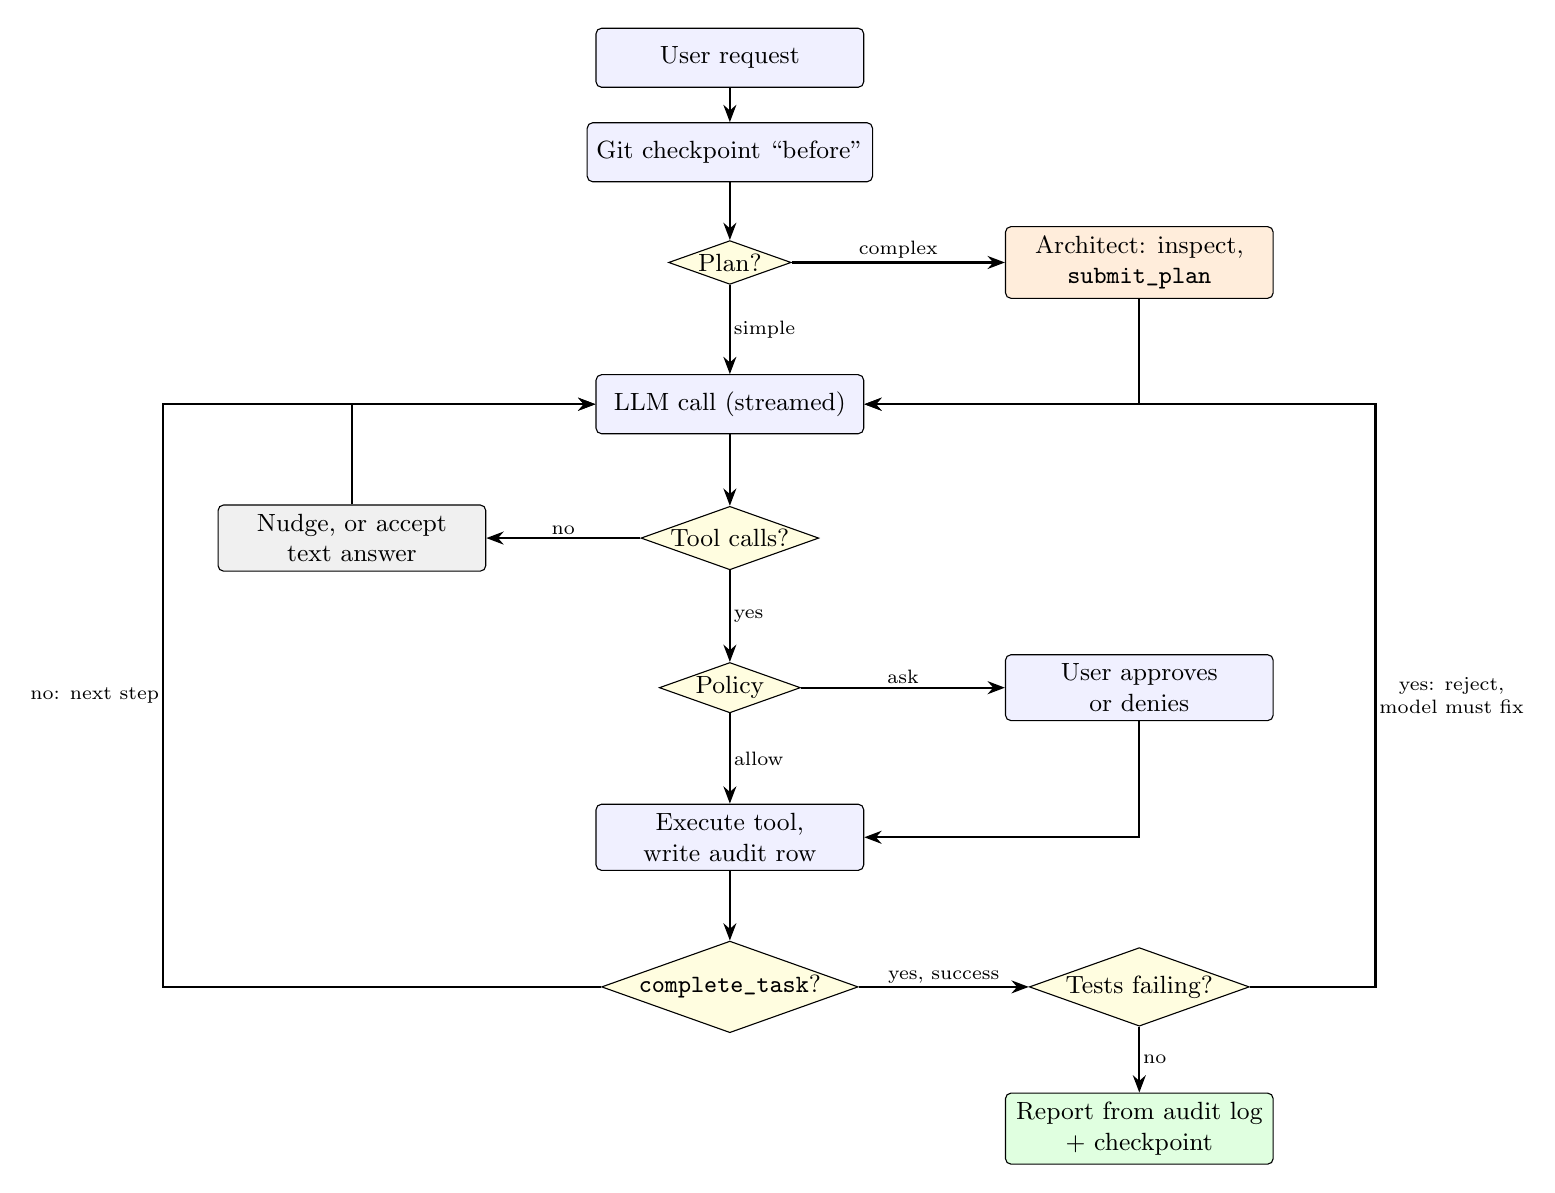
\begin{tikzpicture}[
  font=\small, x=1cm, y=1cm,
  p/.style={draw, rounded corners=2pt, fill=blue!6, align=center, minimum width=34mm, minimum height=7.5mm},
  d/.style={draw, diamond, aspect=2.8, fill=yellow!12, align=center, inner sep=0.5pt},
  arr/.style={-{Stealth[length=2.2mm]}, thick}, lab/.style={font=\scriptsize, fill=white, inner sep=1pt}]
  \node[p] (req) at (0,0) {User request};
  \node[p] (chk) at (0,-1.2) {Git checkpoint ``before''};
  \node[d] (plan) at (0,-2.6) {Plan?};
  \node[p, fill=orange!14] (arch) at (5.2,-2.6) {Architect: inspect,\\\code{submit_plan}};
  \node[p] (llm) at (0,-4.4) {LLM call (streamed)};
  \node[d] (calls) at (0,-6.1) {Tool calls?};
  \node[p, fill=gray!12] (nudge) at (-4.8,-6.1) {Nudge, or accept\\text answer};
  \node[d] (pol) at (0,-8.0) {Policy};
  \node[p] (appr) at (5.2,-8.0) {User approves\\or denies};
  \node[p] (exec) at (0,-9.9) {Execute tool,\\write audit row};
  \node[d] (done) at (0,-11.8) {\code{complete_task}?};
  \node[d] (guard) at (5.2,-11.8) {Tests failing?};
  \node[p, fill=green!12] (rep) at (5.2,-13.6) {Report from audit log\\+ checkpoint};
  \draw[arr] (req)--(chk); \draw[arr] (chk)--(plan);
  \draw[arr] (plan)--node[lab,above]{complex}(arch);
  \draw[arr] (arch.south)|-(llm.east);
  \draw[arr] (plan)--node[lab,right]{simple}(llm);
  \draw[arr] (llm)--(calls);
  \draw[arr] (calls)--node[lab,right]{yes}(pol);
  \draw[arr] (calls)--node[lab,above]{no}(nudge);
  \draw[arr] (nudge.north)|-(llm.west);
  \draw[arr] (pol)--node[lab,above]{ask}(appr);
  \draw[arr] (pol)--node[lab,right]{allow}(exec);
  \draw[arr] (appr.south)|-(exec.east);
  \draw[arr] (exec)--(done);
  \draw[arr] (done)--node[lab,above]{yes, success}(guard);
  \draw[arr] (guard)--node[lab,right]{no}(rep);
  \draw[arr] (done.west)--(-7.2,-11.8)--node[lab,left]{no: next step}(-7.2,-4.4)--(llm.west);
  \draw[arr] (guard.east)--(8.2,-11.8)--node[lab,right,align=center]{yes: reject,\\model must fix}(8.2,-4.4)--(llm.east);
\end{tikzpicture}}
\caption{Simplified control flow. The ``Tests failing?'' guard and the audit-derived report separate ForgeAgent from a plain tool loop. (\emph{Stop} and the step/retry limits apply at every node.)}
\label{fig:loop}
\end{figure}


\subsection{Guards against bad agent behaviour}
\begin{itemize}
  \item \textbf{Verified success.} \code{complete_task(success)} is rejected while the most recent test or build run failed and has not been re-run successfully; the model must fix the problem or report
  \code{partial}.
  \item \textbf{Don't stop at a plan.} A text-only reply that follows edits, or that looks like a plan (``I will\dots'', numbered steps), is answered with a nudge to continue or finish, at most \code{max_nudges} times;
  a plain answer to a question is accepted immediately.
  \item \textbf{Invalid calls are feedback, not crashes.} Unknown tools, malformed JSON and schema violations are returned as errors with the expected schema.
  \item \textbf{Duplicate-action prevention.} A call is fingerprinted by (tool, arguments, \emph{world version}); the world version increments whenever a file or command changes state. A third identical call with no intervening change is refused.
  \item \textbf{Bounded effort.} Step limit per task, retry limit with a changed-approach hint, consecutive-error limit, command timeouts, and process-tree termination on stop.
\end{itemize}

\subsection{Truthful reporting}
The text the user finally reads has two parts: the model's summary and a block \emph{generated by the orchestrator from the \texttt{tool\_runs} table} (files changed, commands executed, last test and build status, checkpoint id).
A model that exaggerates is contradicted by the log shown directly below its claim.

\begin{keyidea}
\textbf{Trust the log, not the narrator.} In any agent that reports on its own work, derive the report from independent evidence (the audit log, a re-run of the tests), and make false success claims
structurally impossible where verification exists.
\end{keyidea}

\subsection{Role prompts}\label{sec:prompts}
The system prompt is assembled from user-editable sections (identity, operating rules, coding standards, planning and testing instructions), a role block, an environment block (operating system, shell, workspace path, date), retrieved memory
and, if the history has been compacted, a progress summary. The operating rules state that file contents, comments, web pages and tool output are untrusted data that cannot alter instructions or permissions, and that analysing code is not executing it.
Tool results that contain third-party content are additionally prefixed with an \emph{untrusted content} notice. No refusal keyword filter exists anywhere in the gateway or orchestrator: model refusal behaviour and execution permission are separate mechanisms.

%==============================================================================================
\section{Persistence, recovery and resume}\label{sec:persist}
\begin{objectives}
Design agent state so that a hard crash loses no completed work and a task can be resumed deterministically.
\end{objectives}

All state needed to continue lives in SQLite (WAL mode \citep{sqlite}): tasks and their statuses (\textsc{pending, planning, running, testing, blocked, failed, completed, cancelled}), the complete message history including tool calls and results,
the audit log, memory, checkpoints and the event timeline. At start-up, any task found in \textsc{planning}, \textsc{running} or \textsc{testing} is, by definition, an orphan of a previous process and is parked as \textsc{blocked} with the message
``Interrupted by application restart'' (Listing~\ref{lst:recover}). \emph{Resume} resets unfinished tasks to \textsc{pending}, reloads their history, adds a message telling the model that the previous run was interrupted and that
it must re-check the workspace rather than assume earlier actions succeeded, and continues. Completed milestones are not repeated.
\lstinputlisting[caption={Crash recovery on start-up (\texttt{backend/app/agent/runtime.py}).},label={lst:recover},basicstyle=\ttfamily\scriptsize]{listings/recover_interrupted.py}

A subtle requirement: if the process dies \emph{between} the model requesting a tool and the result being stored, the history contains a tool call with no result, which most chat templates reject.
\code{repair_tool_pairs} therefore inserts a synthetic result stating that the outcome is unknown (Listing~\ref{lst:pairs}).
\lstinputlisting[caption={Repairing interrupted tool-call pairs (\texttt{backend/app/agent/context.py}).},label={lst:pairs},basicstyle=\ttfamily\scriptsize]{listings/repair_tool_pairs.py}

\begin{figure}[t]
\centering
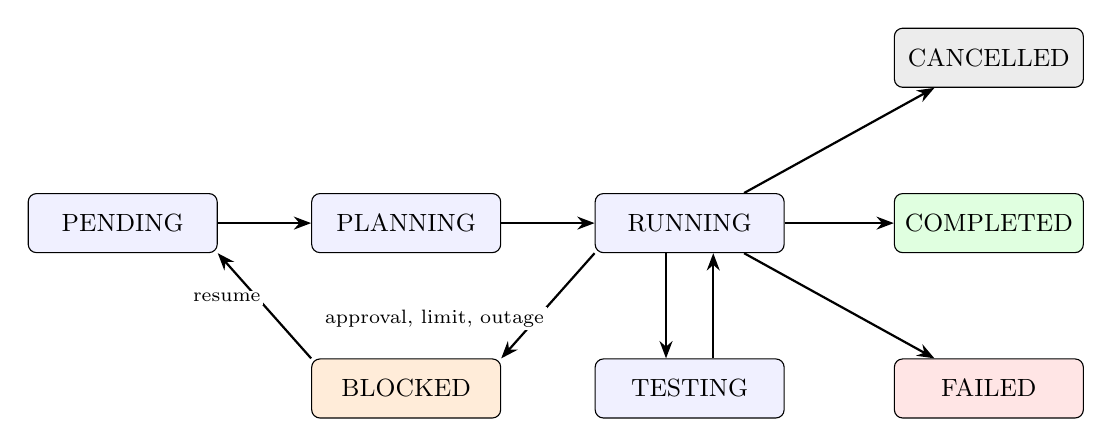
\begin{tikzpicture}[font=\small, x=1cm, y=1cm,
  s/.style={draw, rounded corners=3pt, minimum width=24mm, minimum height=7.5mm, fill=blue!6},
  arr/.style={-{Stealth[length=2.2mm]}, thick}, lab/.style={font=\scriptsize, fill=white, inner sep=1pt}]
  \node[s] (pend) at (0,0) {PENDING};
  \node[s] (plan) at (3.6,0) {PLANNING};
  \node[s] (run) at (7.2,0) {RUNNING};
  \node[s, fill=green!12] (comp) at (11.0,0) {COMPLETED};
  \node[s, fill=red!10] (fail) at (11.0,-2.1) {FAILED};
  \node[s, fill=gray!15] (canc) at (11.0,2.1) {CANCELLED};
  \node[s] (test) at (7.2,-2.1) {TESTING};
  \node[s, fill=orange!15] (blk) at (3.6,-2.1) {BLOCKED};
  \draw[arr] (pend)--(plan); \draw[arr] (plan)--(run); \draw[arr] (run)--(comp);
  \draw[arr] ([xshift=-3mm]run.south) -- ([xshift=-3mm]test.north);
  \draw[arr] ([xshift=3mm]test.north) -- ([xshift=3mm]run.south);
  \draw[arr] (run)--(fail); \draw[arr] (run)--(canc);
  \draw[arr] (run.south west)--node[lab,below left]{approval, limit, outage}(blk.north east);
  \draw[arr] (blk.north west)--node[lab,above left]{resume}(pend.south east);
\end{tikzpicture}
\caption{Task states. \textsc{blocked} covers waiting for approval, step limit, model outage and crash recovery; it is always resumable.}
\label{fig:states}
\end{figure}


%==============================================================================================
\section{Context management}\label{sec:context}
\begin{objectives}
Compute a token budget, and explain truncation and compaction as controlled forgetting.
\end{objectives}

With a 16\,384-token window, the usable prompt budget is
\[
B \;=\; C - R - S_{\text{tools}},\qquad R=\min\!\left(\text{max\_tokens},\,\tfrac{C}{3}\right),
\]
where $C$ is the context size, $R$ the tokens reserved for the reply and $S_{\text{tools}}$ the estimated size of the tool schemas. Token counts are estimated at about $3.6$ characters per token (exact counts are available through llama.cpp's \code{/tokenize} endpoint).
Before each model call the history is estimated; above a threshold (default $0.65\,B$) the older messages are folded into a running summary.

\paragraph{Tool-output truncation.} Outputs longer than a limit are cut head-and-tail and annotated with the \code{tool_run_id}; the full text stays in the audit table and is retrievable with \code{read_full_output}.
\paragraph{Compaction.} The model is asked to summarise the old log (goals, decisions, files changed, real command outcomes, unresolved errors, next steps); on failure a deterministic digest is used. The original user goal is never compacted, and an
assistant tool call is never separated from its results (Listing~\ref{lst:compact}). A last-resort trimmer shortens old tool outputs and drops the oldest complete turns if the prompt still does not fit.
\lstinputlisting[caption={History compaction (\texttt{backend/app/agent/context.py}).},label={lst:compact},basicstyle=\ttfamily\scriptsize]{listings/compact_history.py}

\begin{keyidea}
Compaction is \emph{lossy by design}. Preserve what cannot be re-derived (the goal, decisions, error causes) and discard what can be re-read (file contents, long logs).
\end{keyidea}

%==============================================================================================
\section{Persistent project memory}\label{sec:memory}
Memory items have a kind (requirement, decision, stack, status, completed, pending, error\_fix, file, test, convention, note), a title, content and a \emph{pinned} flag; pinned items are always included in the prompt.
They are written by the agent (\code{remember}), automatically (the request as a requirement, the plan's stack and architecture, completed tasks, and ``failure fixed'' records created when a failing test/build is followed by a pass,
including the files changed in between) and by the user in the Memory tab.

Retrieval needs no embedding model. Text is tokenised (splitting camelCase), uni- and bi-grams are \emph{feature-hashed} \citep{weinberger2009hashing} into a 4096-dimensional signed sparse vector with log-scaled term weights and $L_2$ normalisation (Listing~\ref{lst:embed}),
and relevance is cosine similarity plus a small token-overlap bonus. This is lexical rather than semantic: it finds ``database'' when the memory says ``database'' but not necessarily ``persistence''. A neural embedding model could be substituted behind the same interface.
\lstinputlisting[caption={Feature-hashed vectors (\texttt{backend/app/agent/memory.py}).},label={lst:embed},basicstyle=\ttfamily\scriptsize]{listings/embed.py}

%==============================================================================================
\section{User interface}
The UI (React, TypeScript, Vite, Tailwind CSS, Monaco; bundled locally so it works offline) mirrors the system structure. The \emph{Projects} dashboard (Figure~\ref{fig:1-dashboard.png}) lists workspace, stack, current task, last activity, completion and Git status.
The \emph{Workspace} (Figure~\ref{fig:2-workspace.png}) combines the explorer, editor, a live activity timeline, task, tool, test, checkpoint and memory tabs, and the chat panel with streaming output, approval cards and Stop/Pause controls.
\emph{Settings} (Figure~\ref{fig:4-settings-model.png}) exposes model parameters, server start/stop and model switching, all prompts, autonomy and per-tool permissions, and memory options.

\figscreen{1-dashboard.png}{Projects dashboard.}{0.95}
\figscreen{2-workspace.png}{Workspace after a completed run: explorer, editor, live activity, and the chat panel with the audit-derived ``Verified from tool logs'' block.}{0.98}
\figscreen{4-settings-model.png}{Model and server settings: connection status, capability detection, server start/stop with quantised KV cache, and generation parameters.}{0.75}

%==============================================================================================
\section{Evaluation}\label{sec:eval}
\begin{objectives}
Distinguish unit/integration tests with a scripted model from end-to-end experiments with the real model, and read each result with its limits in mind.
\end{objectives}

\subsection{Automated tests}
The back end has 78 automated tests and the front end 3 (Table~\ref{tab:tests}). The orchestrator tests run the \emph{real} tools, Git and subprocesses against a deterministic fake OpenAI-compatible server that
replays scripted replies, so the control logic, guards and persistence are tested without model variance. All tests pass; the suite was run repeatedly to detect flakiness (see Section~\ref{sec:lessons} for the flakiness this exposed).

\begin{table}[t]
\centering\small
\begin{tabular}{lrl}
\toprule \textbf{File} & \textbf{Tests} & \textbf{What is covered}\\\midrule
\code{test_toolparse.py} & 7 & JSON/XML/fenced tool-call recovery, JSON repair, thinking split\\
\code{test_gateway.py} & 9 & streaming, native calls, fallback, retries, outage, cancel (incl.\ stalled stream)\\
\code{test_security_fs.py} & 31 & path boundaries, junction escape, command classes (incl.\ quote-aware splitting), redaction, file tools, patch (LF/CRLF), Git restore, read-only SQL\\
\code{test_orchestrator.py} & 18 & fix-a-failing-test, success-claim rejection, approvals, stop, duplicates, malformed calls, planning, restart--resume, compaction, step limit\\
\code{test_api.py} & 13 & migrations, projects and workspace validation, files, settings, memory, WebSocket events, queue, checkpoints, timestamp offsets\\
\code{markdown.test.ts} & 3 & HTML escaping of model output, code fences, lists\\\bottomrule
\end{tabular}
\caption{Automated test inventory.}\label{tab:tests}
\end{table}

\subsection{End-to-end experiments with the real model}
All experiments ran on the target machine (RTX 4090 Laptop GPU, 16\,GB VRAM; 64\,GB RAM; Windows~11; llama.cpp build b11620) with the \emph{real} local model, driven through the public HTTP API by \code{scripts/acceptance.py}, which records raw outcomes in \code{docs/ACCEPTANCE_RESULTS.md}. Unless stated otherwise the model was the \texttt{Q4\_K\_M} quantisation with a 16\,384-token context. Scenarios were run once each; this is a demonstration that the mechanisms work end to end, not a statistical estimate of success rates.

\subsubsection*{Acceptance scenarios}
Table~\ref{tab:acc} lists the seven scenarios and the independent evidence for each. \emph{All seven ended in a pass}, but three of them failed or crashed on earlier attempts for reasons described below; those attempts are retained in the raw results file rather than discarded.

\begin{table}[t]
\centering\small
\begin{tabularx}{\linewidth}{llX}
\toprule \textbf{Scenario} & \textbf{Outcome} & \textbf{Independent evidence}\\\midrule
Fix a failing test & pass & tests re-run by the harness after the agent finished: 2 passed; test file byte-identical to the original\\
Workspace boundaries & pass & requested absolute path outside the workspace was refused by the tool; file does not exist on disk\\
Git checkpoint restore & pass & after restoring the ``before'' checkpoint the original content was back and the newly created file was gone\\
Stop a running agent & pass & stop returned in 8.0\,s; task \textsc{cancelled}; no files written in the following 8\,s\\
Supervised approvals & pass (2nd run) & approved edit executed; denied command did not run; audit shows approved/denied per call\\
Restart and resume & pass & backend process killed with \code{taskkill /F} mid-task; recovered as \textsc{blocked}; resumed to \textsc{completed} with all three files\\
Full-stack app & pass & harness re-ran the agent's tests (10 passed) and exercised the live API (201/200/204)\\\bottomrule
\end{tabularx}
\caption{Real-model acceptance scenarios.}\label{tab:acc}
\end{table}

\paragraph{Fix a failing test.} The agent listed the directory, read the source and the test, and edited \code{calc.py} (\code{a - b} $\rightarrow$ \code{a + b}). Its first two \code{run_tests} calls failed because \code{pytest} was not installed in the global interpreter; the agent read the real error, installed it with \code{pip}, re-ran the tests (2 passed), recorded the fix in memory and finished. Nine model steps were used. The first failing runs are visible in the audit log, and the final report states ``Last test run: PASSED'' from that log.

\paragraph{Boundaries.} Asked to write a file at an absolute path outside the workspace, the model called \code{create_file}; the tool refused (``resolves outside the authorized workspace''). The model then tried a shell command, which requested approval and was denied by the harness, and finally created the file inside the workspace as the prompt allowed.

\paragraph{Supervised mode: a failed first attempt that taught something.} The first two runs of this scenario \emph{failed}. The command \code{echo hi > other.txt} was denied and recorded as denied, but the model then created \code{other.txt} with \code{create_file}, which also asked for approval --- and the test script approved every \code{create_file}. The enforcement worked as designed; the test was wrong, and the episode shows that a model \emph{will} try another route after a denial, so every route must pass the same gate. With the script corrected to approve only \code{notes.txt}, the audit log shows: \code{create_file} approved, \code{run_command} denied, \code{create_file} (for \code{other.txt}) denied, and \code{other.txt} did not exist.

\paragraph{Restart and resume.} After the first file was created, the back-end process was killed. A new process started with an empty memory; the task was recovered as \textsc{blocked} with the message ``Interrupted by application restart'', \emph{Resume} was invoked, and the model completed the remaining two files (8--9 steps in total over the two runs). The model call after resumption contained the pre-restart history and the interruption notice.

\subsubsection*{Full-stack application}
The prompt asked for a FastAPI + SQLite Todo application with a static JavaScript front end, a project-local virtual environment, pytest tests, and a live check in the browser. The Architect produced a plan of five milestones plus the automatic review. All seven tasks completed (Table~\ref{tab:fs}); the run used 142 tool calls, of which 14 returned errors that the agent then handled (for example a dev-server port already in use, and a mistaken selector in a browser test). The harness then verified the result \emph{without relying on the agent's report}: the agent's tests passed when re-run (10 passed), and a server started from the workspace answered \code{POST /api/todos} with 201, listed the new item, accepted \code{PATCH} (200) and \code{DELETE} (204), and served an HTML page that uses \code{fetch}.

\begin{table}[t]
\centering\small
\begin{tabular}{llr}
\toprule \textbf{Milestone} & \textbf{Role} & \textbf{Model steps}\\\midrule
Plan: architecture and task breakdown & architect & 3\\
Scaffold project (venv, requirements) & developer & 8\\
Implement FastAPI backend & developer & 30\\
Create static front end & developer & 37\\
Write and run pytest tests & developer & 6\\
Runtime verification in the browser & tester & 19\\
Final review & reviewer & 6\\\bottomrule
\end{tabular}
\caption{Full-stack run: milestones and model steps (Q4\_K\_M).}\label{tab:fs}
\end{table}

\paragraph{This was not a clean run, and we report it as it happened.} The elapsed time of about eight hours is \emph{not} a performance figure. (The harness printed 553 minutes; that number was inflated by a timestamp bug, described in Section~\ref{sec:lessons}, which made browsers and scripts read UTC times as local time.) The elapsed time includes (i) two stalls, of the order of twenty minutes each, in which the agent sat waiting for an approval that the test script was not written to answer --- caused by a classifier false positive on a harmless \code{python -c "...; print(...)"} command (Section~\ref{sec:lessons}) --- one of which a human approved, after which the classifier was fixed in code; (ii) a back-end restart followed by a \emph{Resume} of the same task, which worked; (iii) periods when a second client (the Cline editor extension) was using the same single model and slowed both, from about 7 to about 2.5 tokens/s; and (iv) the test script's own timeouts. Dev servers started by the agent also survived the back-end restart and kept their ports, which made a later \code{start_dev_server} fail with ``port in use''; the agent worked around it, and we list this as a limitation.

\subsection{Quantisation trade-offs: speed, memory and quality}\label{sec:quant}
The 15.4\,GiB \texttt{Q4\_K\_M} file does not fit in 16\,GB of VRAM together with the KV cache, so llama.cpp runs some layers on the CPU. We therefore measured two smaller quantisations of the same model under identical conditions (context 65\,536, KV cache \texttt{q8\_0}, flash attention, one request at a time, nothing else using the GPU): \texttt{IQ4\_XS} (13.4\,GB) and \texttt{IQ3\_S} (11.1\,GB). Each model received the same fixed workload: a 400-token generation, an 7\,318-token prompt, six tool-calling cases with exact expected arguments, and eight coding tasks whose answers were \emph{executed} against hidden tests (the tests were first validated against reference solutions, and a deliberately wrong solution was confirmed to fail). Table~\ref{tab:quant} and Figure~\ref{fig:speed} show the results.

\begin{table}[t]
\centering\small
\begin{tabular}{lrrr}
\toprule & \textbf{Q4\_K\_M} & \textbf{IQ4\_XS} & \textbf{IQ3\_S}\\\midrule
File size (GB) & 15.41 & 13.41 & 11.13\\
VRAM in use (GB) & 13.7 & 13.7 & 13.3\\
Generation (tokens/s) & 7.2 & 9.5 & \textbf{35.9}\\
Prompt processing (tokens/s) & 584 & 677 & \textbf{1195}\\
GPU utilisation (\%) & 30 & 34 & \textbf{94}\\
CPU cores busy (of 32) & 20 & 21 & \textbf{1}\\
Tool calls correct & 6/6 & 6/6 & 6/6\\
Coding tasks passed & 7/8 & 6/8 & 7/8\\
Mean time per coding task (s) & 184 & 137 & \textbf{47}\\\bottomrule
\end{tabular}
\caption{Same model, three quantisations, identical workload (measured). VRAM figures are the whole-GPU reading while the server was busy.}\label{tab:quant}
\end{table}

\begin{figure}[t]
\centering
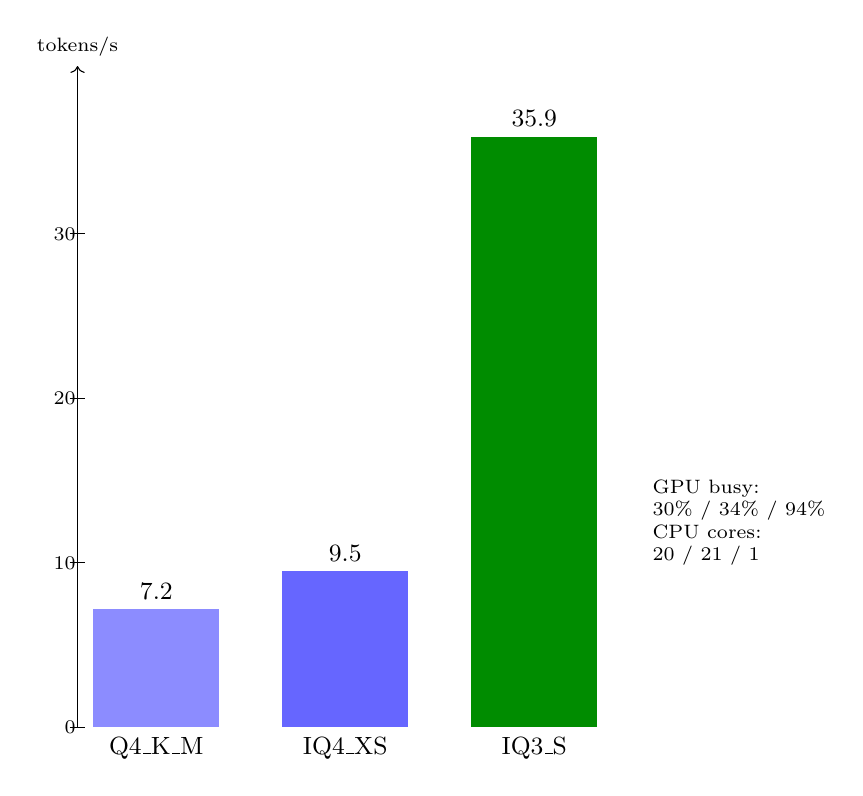
\begin{tikzpicture}[x=1cm,y=1cm,font=\small]
  \def\h{0.095}
  \foreach \name/\v/\c/\x in {Q4\_K\_M/7.2/blue!45/0, IQ4\_XS/9.5/blue!60/2.4, IQ3\_S/35.9/green!55!black/4.8}{
    \fill[\c] (\x,0) rectangle (\x+1.6,\v*\h*2.2);
    \node[above] at (\x+0.8,\v*\h*2.2) {\v};
    \node[below] at (\x+0.8,0) {\name};
  }
  \draw[->] (-0.2,0)--(-0.2,8.4) node[above,font=\scriptsize]{tokens/s};
  \foreach \t in {0,10,20,30}{\draw (-0.3,\t*0.209)--(-0.1,\t*0.209) node[left,font=\scriptsize]{\t};}
  \node[font=\scriptsize,align=left] at (8.2,2.6) {GPU busy:\\30\% / 34\% / 94\%\\CPU cores:\\20 / 21 / 1};
\end{tikzpicture}
\caption{Generation speed in tokens per second (bars drawn to scale). Only IQ3\_S fits entirely in VRAM, which is why the GPU is busy and the CPU idle.}\label{fig:speed}
\end{figure}

\paragraph{Reading the numbers.} Speed is governed by \emph{where the weights live}, not by arithmetic precision alone. With the two larger files part of the model runs on the CPU, so each token waits on the slower processor while the GPU idles (30--34\,\% busy, about 20 CPU cores saturated). \texttt{IQ3\_S} fits completely in VRAM: the GPU is 94\,\% busy, one CPU core is used, and generation is about five times faster. The same effect explains why the dedicated GPU appeared ``not busy'' during the agent runs above.

\paragraph{Quality.} On this small workload the three quantisations were indistinguishable in tool-call reliability (all 6/6) and within one task in coding (7/8, 6/8, 7/8). All three failed the same task, \code{parse_csv_line}, and in every case the recorded finish reason was \code{length}: the model's reasoning consumed the entire 6\,000-token limit before any code was emitted, so the failure reflects the token cap and the long reasoning of this model family, not wrong code. The single genuine logic error was by \texttt{IQ4\_XS} on \code{LRUCache} (a helper class referenced without \code{self.}); the other two solved it. One extra miss in eight tasks is within what chance could produce, and \emph{we draw no conclusion that \texttt{IQ3\_S} is as good as \texttt{Q4\_K\_M} in general}.

\paragraph{Threats to validity.} Eight short tasks, one run each, temperature 0.2, one machine; the tasks are small functions, not repository-scale changes; the full-stack acceptance run used \texttt{Q4\_K\_M} only; and lower-precision quantisations may degrade more on long, multi-step work than these tests can reveal. The practical recommendation that follows is to use \texttt{IQ3\_S} for interactive work where latency dominates and keep \texttt{Q4\_K\_M} available for hard tasks, verifying with the test suite either way.


%==============================================================================================
\section{Engineering lessons}\label{sec:lessons}
Building the system surfaced defects that are instructive beyond this project. Each was found by a test or by running the real model.

\begin{lesson}
\textbf{Stale bytecode defeats fast edit--test loops.} The agent changed \code{a - b} to \code{a + b} (same file size) and re-ran the tests within the same second; Python's \code{.pyc} cache is keyed on source mtime (1\,s resolution) and size, so
the stale bytecode ran and the test still failed. Setting \code{PYTHONDONTWRITEBYTECODE=1} for agent subprocesses fixed it. Autonomous agents create exactly the rapid same-size edits that human workflows rarely do.
\end{lesson}
\begin{lesson}
\textbf{Commit before you respond.} A FastAPI dependency with \code{yield} commits \emph{after} the response is sent. A client that created a project and immediately used it intermittently received 404.
Mutating endpoints now commit explicitly before returning.
\end{lesson}
\begin{lesson}
\textbf{Models write LF; Windows files are CRLF.} \code{git apply} rejected diffs for CRLF files. A strict attempt is followed by a retry with whitespace-tolerant context matching.
\end{lesson}
\begin{lesson}
\textbf{Redaction can break the task.} Redacting \code{password = ...} in everything the model reads made it see \code{[REDACTED]} in the source it was asked to edit. Generic redaction is applied to command output and logs;
for source reads only unmistakable credential formats (private keys, \code{sk-}, \code{ghp_}, AWS keys) are removed.
\end{lesson}
\begin{lesson}
\textbf{Cached collaborators leak between tests.} A shared gateway cached the previous test's fake server and produced order-dependent failures; singletons used in tests must be reset by fixtures.
\end{lesson}
\begin{lesson}
\textbf{Environment first.} In the first real run, the agent correctly diagnosed that \code{pytest} was missing and installed it into the global interpreter. Safe, but poor practice; the default coding standards now instruct it to use a project-local virtual environment.
\end{lesson}
\begin{lesson}
\textbf{Window sizes must agree end to end.} A client that sends a larger prompt than the server's \code{-c} value fails with ``request exceeds the available context''. The context size configured in the application, in the server and in any third-party client must match.
\end{lesson}

%==============================================================================================
\begin{lesson}
\textbf{Parse commands the way the shell does.} The first command classifier split command lines at every \code{;}, including inside quotes, so a harmless \code{python -c "from main import app; print(app.routes)"} was cut into a fragment \code{print(app.routes)}
that was judged an ``unknown command'' and held for approval; the autonomous run then sat waiting. The classifier now splits only outside quotes (and at command substitutions, which genuinely run another command inside double quotes), with regression tests for both the false positive and the cases that must still be caught.
\end{lesson}
\begin{lesson}
\textbf{A denial must close the goal, not one route.} After a shell command was denied, the model achieved the same effect with a file-creation tool. Because every tool passes the same permission gate, the second attempt was also put to the user; the gate, not the model's compliance, is what held. Test scripts that auto-approve must scope approvals narrowly.
\end{lesson}
\begin{lesson}
\textbf{Never emit timezone-naive timestamps.} SQLite returns naive datetimes; the API sent them without an offset, so a browser in UTC+1 displayed ``1 h ago'' for something that had just happened, and the test harness computed inflated durations. All timestamps are now serialised with an explicit UTC offset, with a regression test.
\end{lesson}
\begin{lesson}
\textbf{Stalled-on-approval must be visible.} An autonomous agent that needs a human decision looks identical to a slow one. The UI shows an approval card and the task status \textsc{blocked}; automated test harnesses must watch for pending approvals explicitly.
\end{lesson}
\begin{lesson}
\textbf{Idle GPU does not mean unused GPU.} During generation with part of the model on the CPU the GPU showed 2--39\,\% utilisation although the weights were mostly in VRAM; the processors alternate, and the CPU side sets the pace. Measuring GPU/CPU utilisation together with throughput (Section~\ref{sec:quant}) showed that choosing a quantisation that fits entirely in VRAM was worth more than any software optimisation.
\end{lesson}

\section{Limitations and threats to validity}\label{sec:limits}
\begin{itemize}
  \item \textbf{Not a sandbox.} Commands run with the user's account rights; the classifier is a heuristic. No Docker/WSL2 isolation is integrated.
  \item \textbf{Small sample.} The end-to-end experiments use a handful of tasks on one model and one machine; they demonstrate that mechanisms work, not their success rate. We do not report SWE-bench or HumanEval \citep{chen2021codex} results.
  \item \textbf{Model dependence.} Results depend on the chosen quantised model; some community models are modified to refuse less \citep{arditi2024refusal}, which shifts risk toward the permission layer.
  \item \textbf{Prompt injection is mitigated, not solved.} Labelling and least privilege reduce impact; a determined injection that leads the user to approve a harmful action is possible. We did not run an injection benchmark such as AgentDojo \citep{debenedetti2024agentdojo}.
  \item \textbf{Lexical memory.} Feature-hashed retrieval has no semantic generalisation.
  \item \textbf{Throughput.} About 8--13 tokens/s with partial CPU offload makes large builds slow; the text-only model cannot inspect screenshots (it uses DOM text and console/network errors).
  \item \textbf{Orphaned dev servers.} Servers started by the agent are children of the back-end process tree only while it runs; after a hard restart they keep running and hold their ports, so a later \code{start_dev_server} can fail with ``port in use''. Tracking and reaping them on recovery is future work.
  \item \textbf{Shared model.} Any other client of the same local server (an editor extension, a second application) competes for the single model and can cut throughput several-fold; ForgeAgent serialises its own calls but cannot control others.
  \item \textbf{Single user, single machine}; one active run per project; inference is serialised.
\end{itemize}

\section{Conclusion and future work}
ForgeAgent shows that a locally hosted 27B model can drive a complete software-engineering workflow when the surrounding system supplies what the model lacks: tolerant parsing of its output, enforced permissions, independent verification, durable state and disciplined context use.
Future work: OS-level isolation (WSL2/containers); neural embeddings; an injection benchmark; speculative decoding or smaller specialised models for speed; multi-model role assignment on larger hardware; and a systematic evaluation on public benchmarks.

\section*{Availability}
Source code, tests, installation scripts, screenshots and raw acceptance results: \url{https://github.com/bahdleen/forgeagent} (MIT licence).

\appendix
\section{Reproducing the results}
\begin{enumerate}[nosep]
  \item Install prerequisites (Python 3.12, Node 20, Git for Windows, NVIDIA driver) and run \code{scripts\install.ps1 -InstallLlama -DownloadModel}.
  \item Start with \code{scripts\start.ps1 -WithLlama}; verify the status bar shows the model.
  \item Tests: \code{cd backend; .venv\Scripts\python -m pytest}; \code{cd frontend; npm test}.
  \item Real-model scenarios: \code{python scripts\acceptance.py <scenario>} with scenario one of \code{fix_test, boundaries, checkpoint, stop, supervised, resume, fullstack}; output is appended to \code{docs/ACCEPTANCE_RESULTS.md}.
\end{enumerate}

\section{Exercises}
\begin{exercise}[title={Exercises (with hints)}]
\begin{enumerate}[nosep]
  \item \emph{Tool design.} Add a \code{http_get} tool restricted to \texttt{localhost}. Which permission category and which classifier rules does it need? (Hint: Section~\ref{sec:tools}.)
  \item \emph{Guard.} Extend the completion guard so that \code{success} is also rejected when the build was never run in a project that has a \code{build} script. What are the false-positive risks?
  \item \emph{Budget.} For $C=32\,768$, \code{max_tokens}$=4096$ and $S_{\text{tools}}=3500$, compute $B$ and the compaction trigger. How does the KV-cache cost change relative to $C=16\,384$?
  \item \emph{Recovery.} Write a test that kills the back end between a tool call and its result and show that \code{repair_tool_pairs} is exercised. (Hint: Listing~\ref{lst:pairs}.)
  \item \emph{Security.} Construct a command that the classifier marks ``auto'' but that writes outside the workspace. Propose a fix; then explain why a fix at this layer can never be complete.
  \item \emph{Memory.} Replace feature hashing by a neural embedding endpoint behind the same \code{embed} interface and compare retrieval for ``persistence'' vs.\ ``database''.
\end{enumerate}
\end{exercise}

\section{Glossary}
\begin{description}[nosep,style=nextline]
  \item[Agent loop] Repeating model call $\rightarrow$ tool execution $\rightarrow$ observation until a stop condition.
  \item[GGUF] File format used by llama.cpp for (quantised) model weights.
  \item[KV cache] Stored attention keys/values for previous tokens; grows with context length.
  \item[Compaction] Replacing old conversation with a shorter summary.
  \item[Least privilege] Giving a component only the permissions its task needs \citep{saltzer1975protection}.
  \item[Prompt injection] Instructions hidden in data that try to redirect a model \citep{greshake2023indirect}.
\end{description}

\bibliographystyle{plainnat}
\bibliography{references}

\end{document}
